\documentclass[11pt,compress,t,notes=noshow, aspectratio=169, xcolor=table]{beamer}

\usepackage{../../style/lmu-lecture}
% Defines macros and environments
% This file is included in slides and exercises

% Rarely used fontstyle for R packages, used only in 
% - forests/slides-forests-benchmark.tex
% - exercises/single-exercises/methods_l_1.Rnw
% - slides/cart/attic/slides_extra_trees.Rnw
\newcommand{\pkg}[1]{{\fontseries{b}\selectfont #1}}

% Spacing helpers, used often (mostly in exercises for \dlz)
\newcommand{\lz}{\vspace{0.5cm}} % vertical space (used often in slides)
\newcommand{\dlz}{\vspace{1cm}}  % double vertical space (used often in exercises, never in slides)
\newcommand{\oneliner}[1] % Oneliner for important statements, used e.g. in iml, algods
{\begin{block}{}\begin{center}\begin{Large}#1\end{Large}\end{center}\end{block}}

% Don't know if this is used or needed, remove?
% textcolor that works in mathmode
% https://tex.stackexchange.com/a/261480
% Used e.g. in forests/slides-forests-bagging.tex
% [...] \textcolor{blue}{\tfrac{1}{M}\sum^M_{m} [...]
% \makeatletter
% \renewcommand*{\@textcolor}[3]{%
%   \protect\leavevmode
%   \begingroup
%     \color#1{#2}#3%
%   \endgroup
% }
% \makeatother


\title{Applied Machine Learning}
% \author{LMU}
%\institute{\href{https://compstat-lmu.github.io/lecture_iml/}{compstat-lmu.github.io/lecture\_iml}}
\date{}

\begin{document}

\newcommand{\titlefigure}{figure/empty}
\newcommand{\learninggoals}{
\item old material
\item also check \textbf{imbalanced-learning} slides in \textbf{lecture\_advml} repo}

\lecturechapter{Applied Performance Evaluation}
\lecture{Applied Machine Learning}


\begin{frame}[fragile]{Dealing with imbalanced data}
\phantomsection\label{dealing-with-imbalanced-data}
We train a classification tree to predict a quite imbalanced binary
classification task with a very small, but very import class.

\scriptsize

\begin{verbatim}
##   acc   bac   tpr   fpr   auc 
## 0.973 0.806 0.988 0.375 0.874
\end{verbatim}

\begin{center}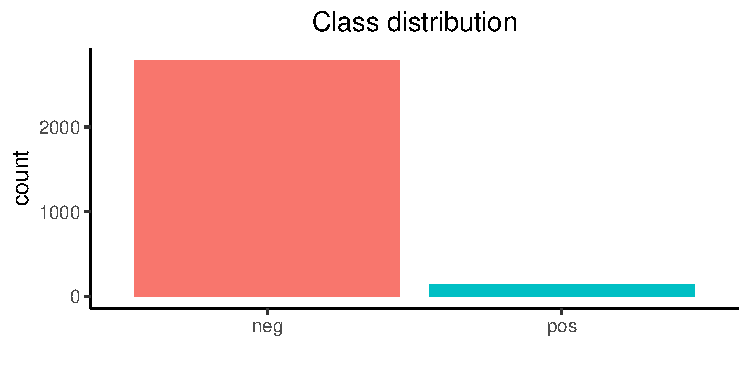
\includegraphics[width=0.7\textwidth]{figure/unnamed-chunk-3-1} \end{center}

\begin{verbatim}
##         predicted
## true     neg pos -err.-
##   neg    554   7      7
##   pos      9  15      9
##   -err.-   9   7     16
\end{verbatim}

\normalsize
\end{frame}

\begin{frame}{Dealing with imbalanced data}
\phantomsection\label{dealing-with-imbalanced-data-1}
Measures like balanced accuracy (BAC) or F1 score might enable adequate
evaluation of models on imbalanced data.

But many learners tend to produce unsatisfactory results in these
situations. What can be done?

\begin{enumerate}
\tightlist
\item
  Try different algorithms: trees, for example, often perform well on
  imbalanced datasets
\end{enumerate}
\end{frame}

\begin{frame}{Threshold Tuning (I)}
\phantomsection\label{threshold-tuning-i}
\begin{enumerate}
\setcounter{enumi}{1}
\tightlist
\item
  Do Threshold Tuning
\end{enumerate}

\begin{itemize}
\tightlist
\item
  If a classifier outputs probabilities \(\pi (x)\) (or scores
  \(f(x)\)), they are transformed into labels by comparing it to a
  threshold:
\end{itemize}

\[
\hat y = 1 \quad \text{if} \quad \pi (x) > \alpha
\]

\begin{itemize}
\tightlist
\item
  For probabilities, this threshold is often set to \(0.5\) per default
  (or \(0\) for scores)
\end{itemize}
\end{frame}

\begin{frame}{Threshold Tuning (II)}
\phantomsection\label{threshold-tuning-ii}
In this example, a threshold of \(0.5\) is a bad choice
(\(FPR = 0, TPR = 0\)).

\begin{center}
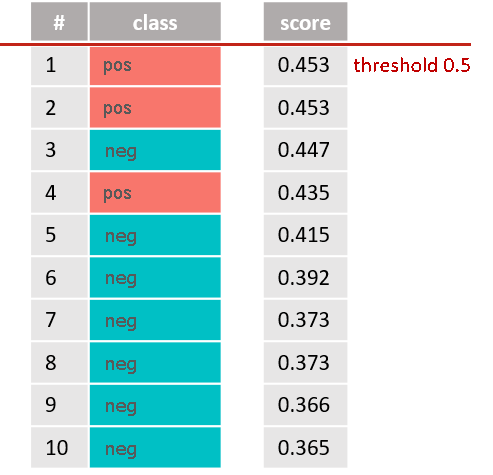
\includegraphics[width=0.45\textwidth]{figure/threshold_tuning11.png}
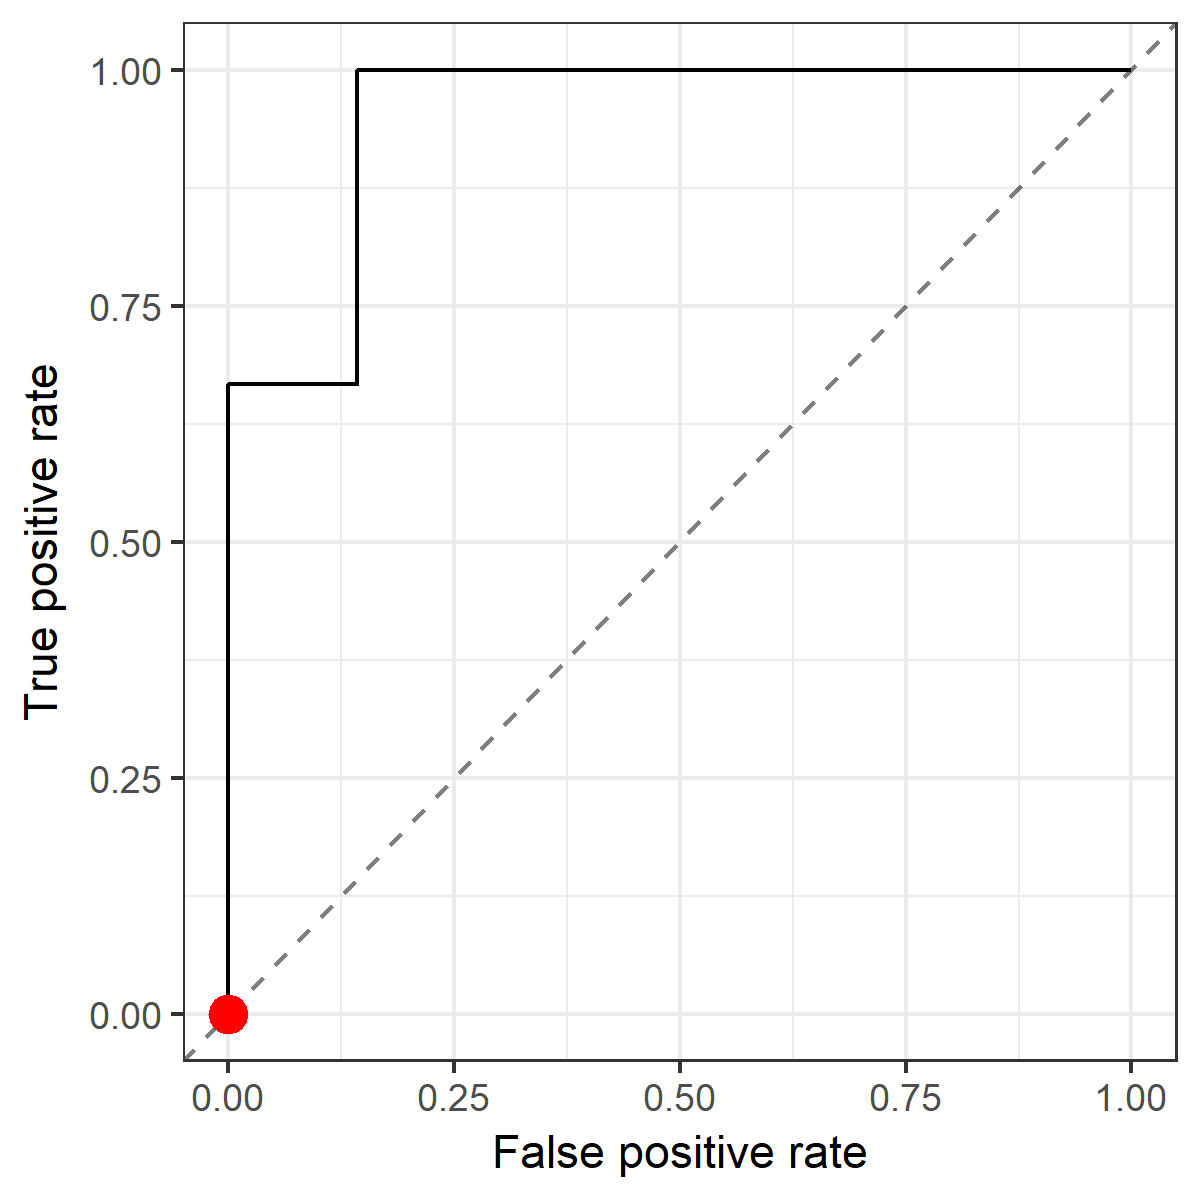
\includegraphics[width=0.45\textwidth]{figure/threshold_tuning12.png}
\end{center}
\end{frame}

\begin{frame}{Threshold Tuning (III)}
\phantomsection\label{threshold-tuning-iii}
\begin{itemize}
\tightlist
\item
  However, this threshold can be anything between \(0\) and \(1\).
\item
  When adjusting the threshold, we can control the number of examples
  labeled true
\item
  Naive way: Calculate labels for every possible threshold, evaluate and
  choose your favorite threshold
\item
  Better: Look at the ROC curve, where each point corresponds to the TPR
  and FPR for one specific threshold and take the one you prefer
\end{itemize}
\end{frame}

\begin{frame}{Threshold Tuning (IV)}
\phantomsection\label{threshold-tuning-iv}
In this simple artificial example, we can achieve a much better
performance (FPR = \(0.143\), TPR = \(1\)) by setting thresholds
appropriately.

\begin{center}
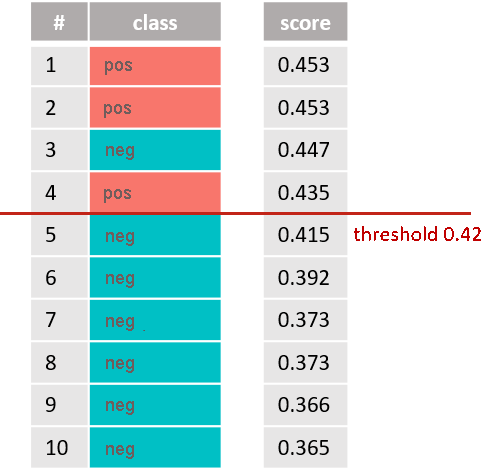
\includegraphics[width=0.45\textwidth]{figure/threshold_tuning21.png}
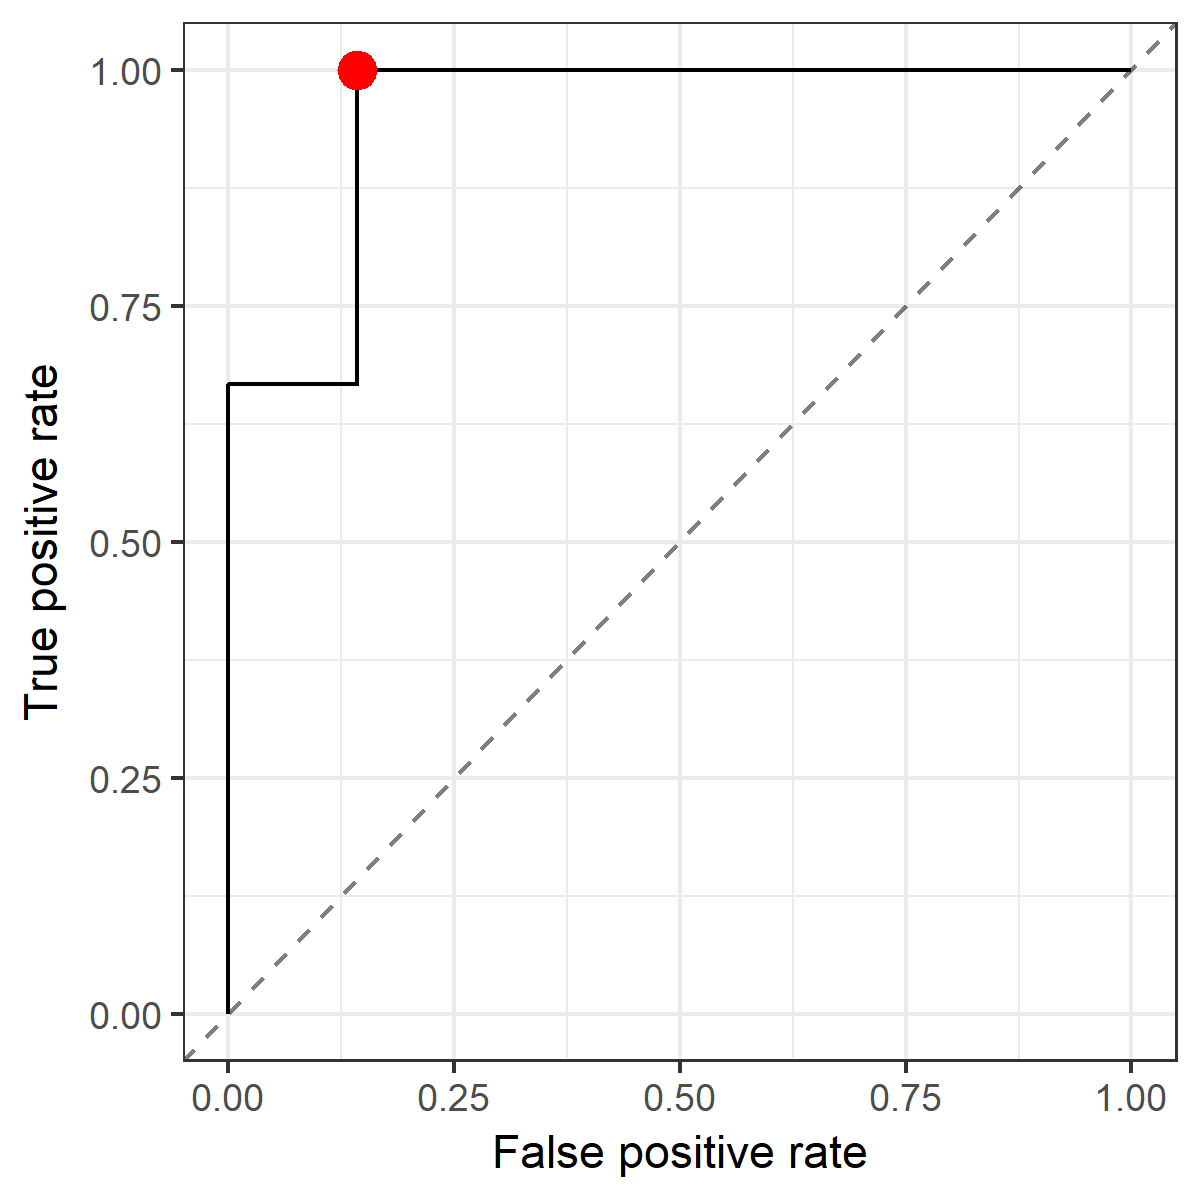
\includegraphics[width=0.45\textwidth]{figure/threshold_tuning22.png}
\end{center}
\end{frame}

\begin{frame}{Over- and undersampling}
\phantomsection\label{over--and-undersampling}
\begin{enumerate}
\setcounter{enumi}{2}
\tightlist
\item
  Try to improve the class distribution

  \begin{itemize}
  \tightlist
  \item
    if possible, collect more data
  \item
    try to modify your data to improve the class distribution via

    \begin{itemize}
    \tightlist
    \item
      oversampling
    \item
      undersampling
    \item
      SMOTE
    \end{itemize}
  \end{itemize}
\end{enumerate}
\end{frame}

\begin{frame}{Oversampling (I)}
\phantomsection\label{oversampling-i}
One approach to balance the class distribution is \textbf{oversampling}:
We randomly add copies from the underrepresented class.

\begin{center}
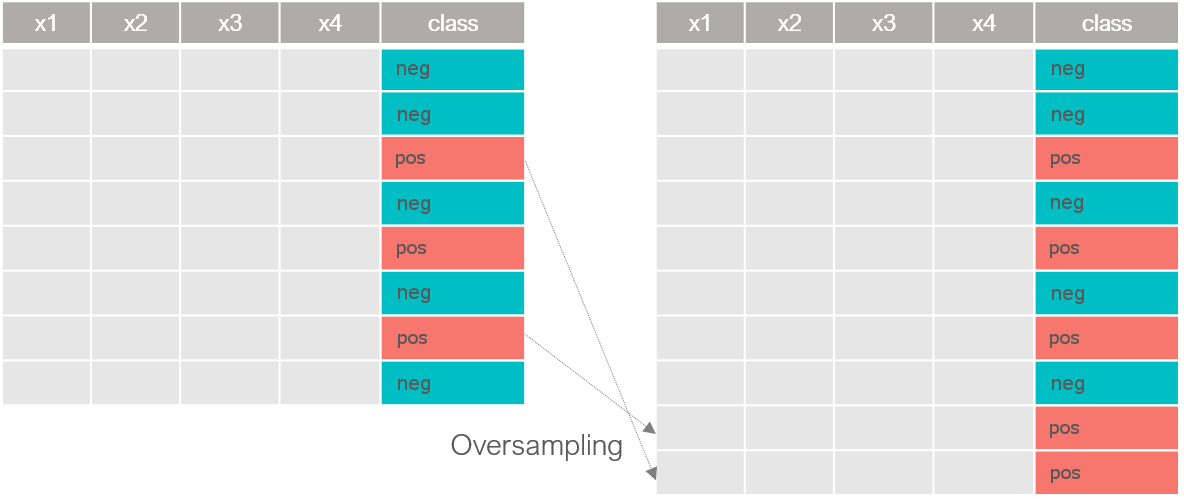
\includegraphics{figure/oversampling.png}
\end{center}
\end{frame}

\begin{frame}{Oversampling (II)}
\phantomsection\label{oversampling-ii}
The number of copies we add by oversampling is specified by a
\textbf{oversampling rate}. If the oversampling rate is \(2\), the
underrepresented class gets doubled.

\scriptsize

\begin{center}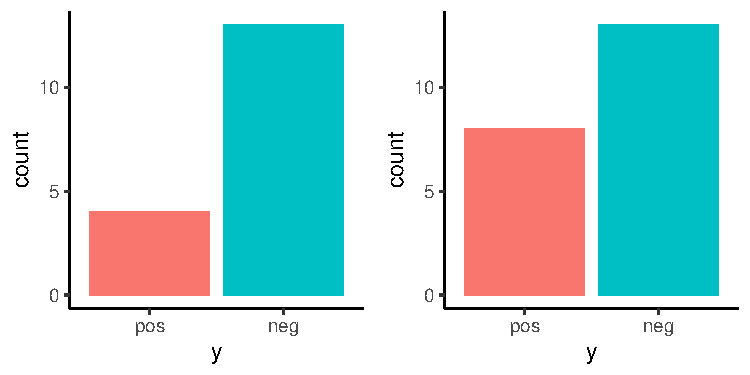
\includegraphics[width=0.7\textwidth]{figure/unnamed-chunk-4-1} \end{center}

\normalsize
\end{frame}

\begin{frame}{Oversampling (III)}
\phantomsection\label{oversampling-iii}
\textbf{Pros}:

\begin{itemize}
\tightlist
\item
  Oversampling is easy to implement
\item
  All information available is used
\end{itemize}

\textbf{Cons}:

\begin{itemize}
\tightlist
\item
  The size of the dataset increases which might increase runtime of the
  training or cause storage problems
\item
  It increases the likelihood of overfitting since the minority class
  events are replicated
\end{itemize}
\end{frame}

\begin{frame}{Undersampling (I)}
\phantomsection\label{undersampling-i}
Another is \textbf{undersampling}: We randomly \textbf{throw away}
observations from the overrepresented class.

\begin{center}
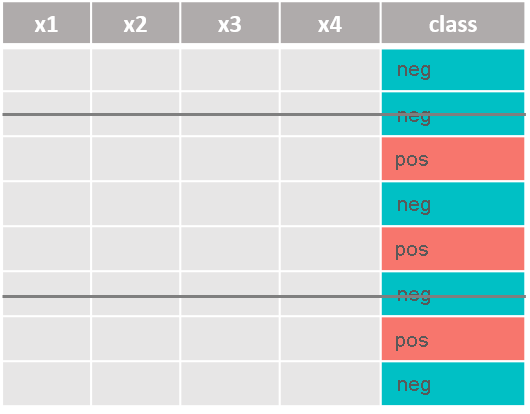
\includegraphics[width = 0.5\linewidth]{figure/undersampling.png}
\end{center}
\end{frame}

\begin{frame}{Undersampling (II)}
\phantomsection\label{undersampling-ii}
Again, the number of majority class observations we delete is specified
by a \textbf{undersampling rate}. If the rate is \(\frac{1}{2}\), the
overrepresented class gets halved.

\scriptsize

\begin{center}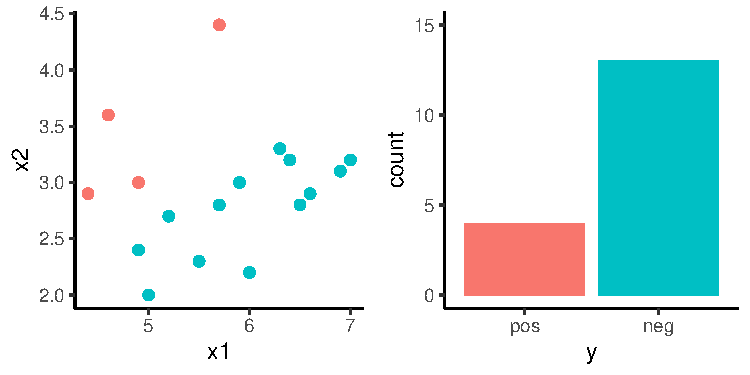
\includegraphics[width=0.7\textwidth]{figure/unnamed-chunk-5-1} \end{center}

\normalsize
\end{frame}

\begin{frame}{Undersampling (III)}
\phantomsection\label{undersampling-iii}
The number of majority class observations we delete is specified by a
\textbf{undersampling rate}. If the rate is \(\frac{1}{2}\), the
overrepresented class gets halved.

\scriptsize

\begin{center}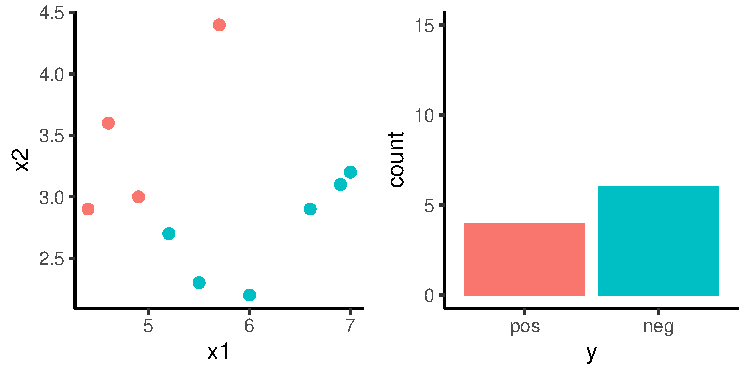
\includegraphics[width=0.7\textwidth]{figure/unnamed-chunk-6-1} \end{center}

\normalsize
\end{frame}

\begin{frame}{Undersampling (IV)}
\phantomsection\label{undersampling-iv}
\textbf{Pros}:

\begin{itemize}
\tightlist
\item
  Undersampling is also easy to implement
\item
  It can help improve runtime and storage problems by reducing the
  number of training data samples (when the training data set is huge)
\end{itemize}

\textbf{Cons}:

\begin{itemize}
\tightlist
\item
  We loose information by throwing away data samples
\end{itemize}
\end{frame}

\begin{frame}{SMOTE (I)}
\phantomsection\label{smote-i}
Both oversampling (duplicating examples) and undersampling (throwing
away data) might be problematic. Instead we might prefer to generate
\textbf{new synthetic} examples.

We generate new synthetic examples using \textbf{SMOTE} algorithm:

\begin{itemize}
\tightlist
\item
  For each original data point \(x\), find the \(k\) nearest neighbors
\item
  Then repeat \(N - 1\) times:

  \begin{itemize}
  \tightlist
  \item
    randomly select one of the \(k\) nearest neighbors, called
    \(\tilde x\)
  \item
    randomly interpolate \(x\) and \(\tilde x\) to create a new
    observation
  \end{itemize}
\item
  The number of artificial data points is defined by the \textbf{rate}
  \(N\) (\(N = 2\) means that the minority class gets doubled)
\end{itemize}
\end{frame}

\begin{frame}{SMOTE (II)}
\phantomsection\label{smote-ii}
Connect each minority class point to its \(k\) (here: \(k = 2\)) nearest
neighbors.

\scriptsize

\begin{center}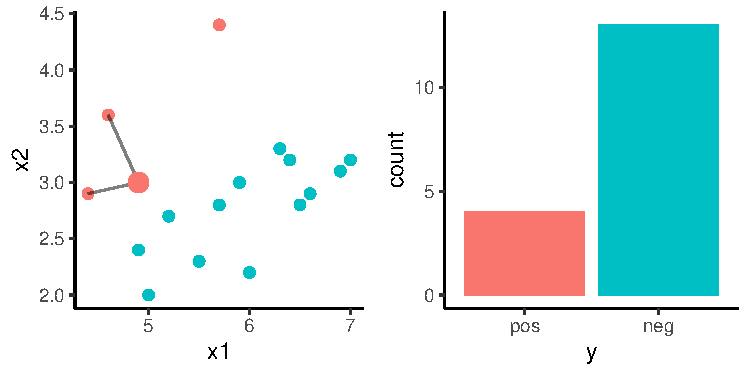
\includegraphics[width=0.7\textwidth]{figure/unnamed-chunk-8-1} \end{center}

\normalsize
\end{frame}

\begin{frame}{SMOTE (III)}
\phantomsection\label{smote-iii}
Randomly select a neighbor and generate a new point by selecting a
random point lying on the respective connection.

\scriptsize

\begin{center}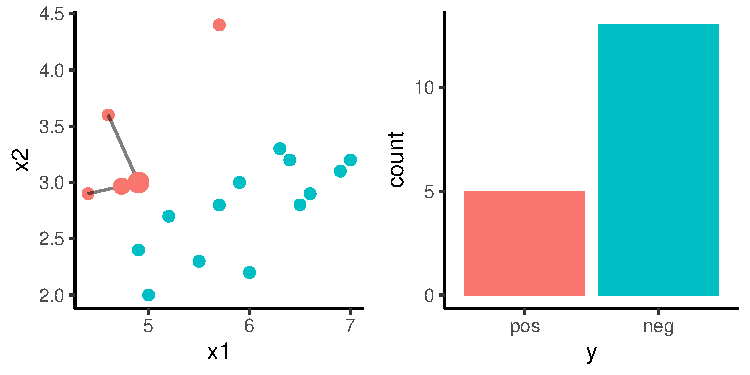
\includegraphics[width=0.7\textwidth]{figure/unnamed-chunk-9-1} \end{center}

\normalsize
\end{frame}

\begin{frame}{SMOTE (IV)}
\phantomsection\label{smote-iv}
For each of the minority class points, repeat the above procedure
\(N - 1\) times.

\scriptsize

\begin{center}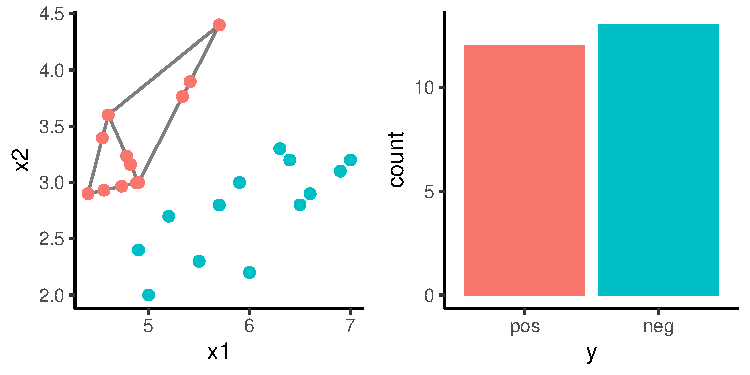
\includegraphics[width=0.7\textwidth]{figure/unnamed-chunk-10-1} \end{center}

\normalsize
\end{frame}

\begin{frame}{SMOTE (V)}
\phantomsection\label{smote-v}
The original SMOTE algorithm cannot handle categorical features, but the
algorithm can be extended:

\begin{itemize}
\tightlist
\item
  To determine the nearest neighbors, use a distance that can handle
  categorical variables (e.g., Gower distance)
\item
  Instead of interpolation between between two factor levels, we
  randomly take one of them.
\end{itemize}

\textbf{Note} that each time the data is modified (especially for SMOTE,
over- and undersampling) hyperparameters of used machine learning
algorithms possibly need to be changed!
\end{frame}

\begin{frame}{Example (I)}
\phantomsection\label{example-i}
Let's return to the example from the beginning. We try to improve
performance by using over- and undersampling as well as the SMOTE
algorithm.

For undersampling we use a rate or \(\frac{1}{20}\), for oversampling a
rate of \(20\) and for SMOTE, we also use a rate of \(20\) and set the
number of nearest neighbors to \(k = 3\).
\end{frame}

\begin{frame}[fragile]{Example (II)}
\phantomsection\label{example-ii}
Evaluation is again done via holdout (\(80\%\) for training, \(20\%\)
for testing). Here, all methods reduce the FPR while, at the same time,
the TPR worsens.

\scriptsize

\begin{verbatim}
##     acc   bac   tpr   fpr   auc        method
## 1 0.973 0.806 0.988 0.375 0.874    imbalanced
## 2 0.916 0.857 0.922 0.208 0.868  oversampling
## 3 0.863 0.849 0.865 0.167 0.856 undersampling
## 4 0.964 0.882 0.971 0.208 0.898         SMOTE
\end{verbatim}

\normalsize
\end{frame}

\begin{frame}{Imbalanced data: Change perspective}
\phantomsection\label{imbalanced-data-change-perspective}
If none of the above approaches worked, you may have to take on another
perspective.

\begin{enumerate}
\setcounter{enumi}{3}
\tightlist
\item
  Try a different perspective: use \textbf{anomaly} or \textbf{change
  detection} techniques instead of classification algorithms
\end{enumerate}

\begin{center}
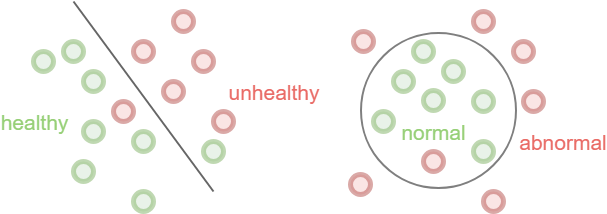
\includegraphics[width=0.8\textwidth]{figure/classification-vs-anomaly.png}
\end{center}
\end{frame}


\endlecture
\end{document}
